\documentclass{standalone}
\usepackage{tikz}
\usetikzlibrary{patterns, positioning}

\begin{document}
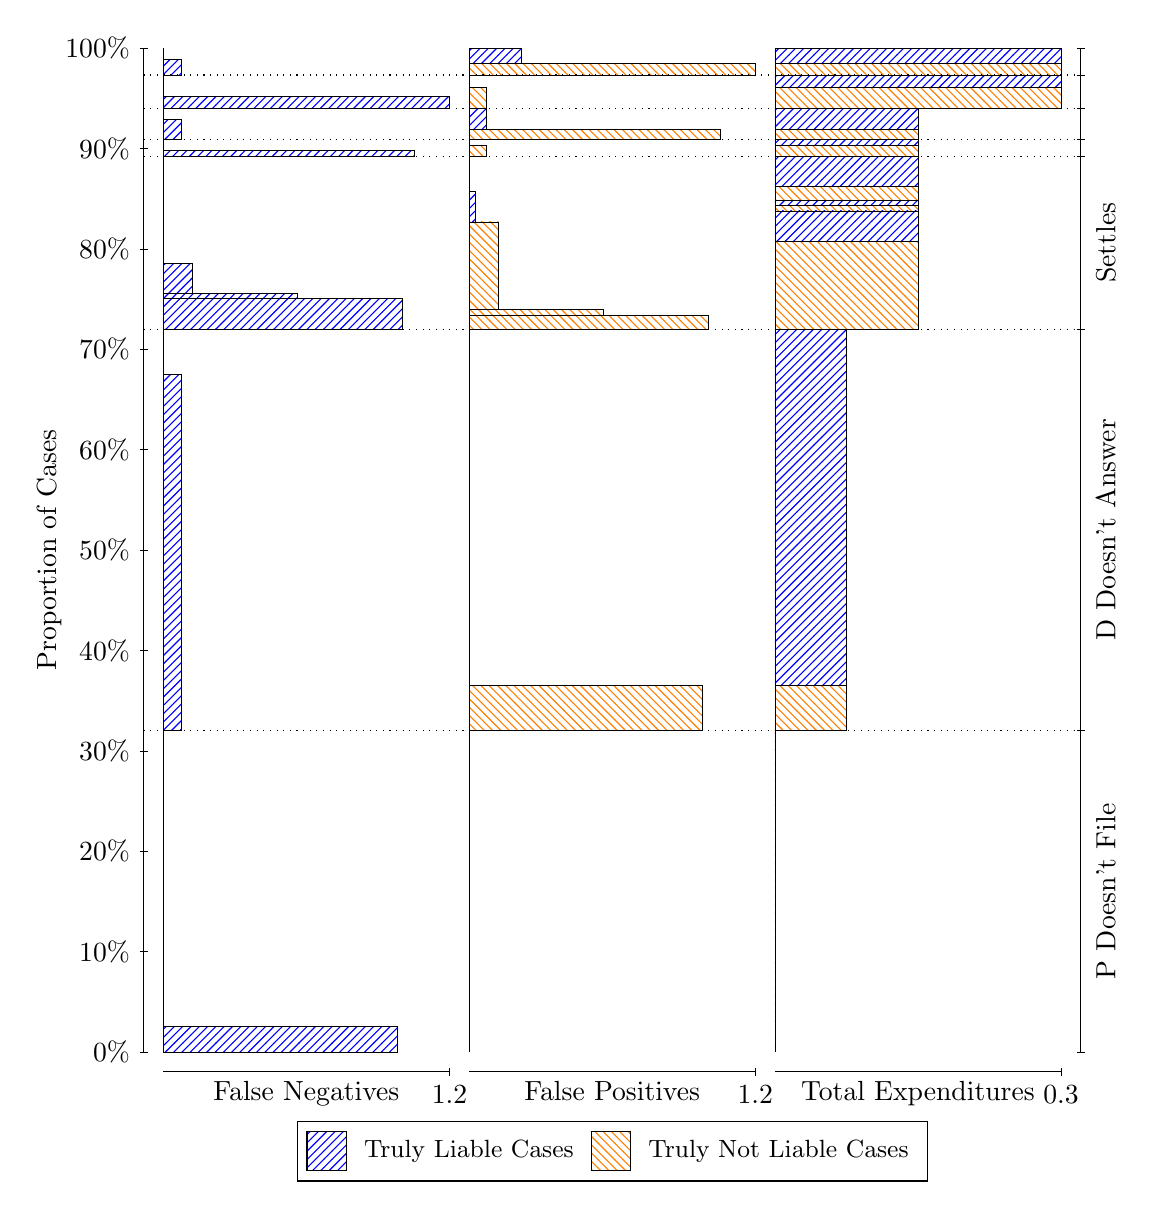
\begin{tikzpicture}
\draw[black, very thin] (1.5,1.75) -- (1.5,14.5);
\node[rotate=90, anchor=center] at (0.3, 8.125) {Proportion of Cases};
\draw[black, very thin] (1.45,1.75) -- (1.55,1.75);
\node[anchor=east] at (1.45, 1.75) {0\%};
\draw[black, very thin] (1.45,3.025) -- (1.55,3.025);
\node[anchor=east] at (1.45, 3.025) {10\%};
\draw[black, very thin] (1.45,4.3) -- (1.55,4.3);
\node[anchor=east] at (1.45, 4.3) {20\%};
\draw[black, very thin] (1.45,5.575) -- (1.55,5.575);
\node[anchor=east] at (1.45, 5.575) {30\%};
\draw[black, very thin] (1.45,6.85) -- (1.55,6.85);
\node[anchor=east] at (1.45, 6.85) {40\%};
\draw[black, very thin] (1.45,8.125) -- (1.55,8.125);
\node[anchor=east] at (1.45, 8.125) {50\%};
\draw[black, very thin] (1.45,9.4) -- (1.55,9.4);
\node[anchor=east] at (1.45, 9.4) {60\%};
\draw[black, very thin] (1.45,10.675) -- (1.55,10.675);
\node[anchor=east] at (1.45, 10.675) {70\%};
\draw[black, very thin] (1.45,11.95) -- (1.55,11.95);
\node[anchor=east] at (1.45, 11.95) {80\%};
\draw[black, very thin] (1.45,13.225) -- (1.55,13.225);
\node[anchor=east] at (1.45, 13.225) {90\%};
\draw[black, very thin] (1.45,14.5) -- (1.55,14.5);
\node[anchor=east] at (1.45, 14.5) {100\%};

\draw[black, very thin] (13.4,1.75) -- (13.4,14.5);
\draw[black, very thin] (13.35,1.75) -- (13.45,1.75);
\node[anchor=west] at (13.35, 1.75) {};
\draw[black, very thin] (13.35,5.832) -- (13.45,5.832);
\node[anchor=west] at (13.35, 5.832) {};
\draw[black, very thin] (13.35,10.929) -- (13.45,10.929);
\node[anchor=west] at (13.35, 10.929) {};
\draw[black, very thin] (13.35,13.128) -- (13.45,13.128);
\node[anchor=west] at (13.35, 13.128) {};
\draw[black, very thin] (13.35,13.336) -- (13.45,13.336);
\node[anchor=west] at (13.35, 13.336) {};
\draw[black, very thin] (13.35,13.729) -- (13.45,13.729);
\node[anchor=west] at (13.35, 13.729) {};
\draw[black, very thin] (13.35,14.157) -- (13.45,14.157);
\node[anchor=west] at (13.35, 14.157) {};
\draw[black, very thin] (13.35,14.5) -- (13.45,14.5);
\node[anchor=west] at (13.35, 14.5) {};

\draw[black, very thin, pattern color=blue, pattern=north east lines] (1.75,1.75) rectangle (4.716,2.0755);
\draw[black, very thin, pattern color=orange, pattern=north west lines] (1.75,2.0755) rectangle (1.75,5.832);
\draw[black, very thin, pattern color=blue, pattern=north east lines] (1.75,5.832) rectangle (1.9724,10.358);
\draw[black, very thin, pattern color=orange, pattern=north west lines] (1.75,10.358) rectangle (1.75,10.929);
\draw[black, very thin, pattern color=blue, pattern=north east lines] (1.75,10.929) rectangle (4.7901,11.32);
\draw[black, very thin, pattern color=blue, pattern=north east lines] (1.75,11.32) rectangle (3.4554,11.381);
\draw[black, very thin, pattern color=blue, pattern=north east lines] (1.75,11.381) rectangle (2.1207,11.765);
\draw[black, very thin, pattern color=orange, pattern=north west lines] (1.75,11.765) rectangle (1.75,13.128);
\draw[black, very thin, pattern color=blue, pattern=north east lines] (1.75,13.128) rectangle (4.9384,13.198);
\draw[black, very thin, pattern color=orange, pattern=north west lines] (1.75,13.198) rectangle (1.75,13.336);
\draw[black, very thin, pattern color=blue, pattern=north east lines] (1.75,13.336) rectangle (1.9724,13.593);
\draw[black, very thin, pattern color=orange, pattern=north west lines] (1.75,13.593) rectangle (1.75,13.729);
\draw[black, very thin, pattern color=blue, pattern=north east lines] (1.75,13.729) rectangle (5.3833,13.889);
\draw[black, very thin, pattern color=orange, pattern=north west lines] (1.75,13.889) rectangle (1.75,14.157);
\draw[black, very thin, pattern color=blue, pattern=north east lines] (1.75,14.157) rectangle (1.9724,14.355);
\draw[black, very thin, pattern color=orange, pattern=north west lines] (1.75,14.355) rectangle (1.75,14.5);
\draw[black, very thin, pattern color=orange, pattern=north west lines] (5.6333,1.75) rectangle (5.6333,5.5066);
\draw[black, very thin, pattern color=blue, pattern=north east lines] (5.6333,5.5066) rectangle (5.6333,5.832);
\draw[black, very thin, pattern color=orange, pattern=north west lines] (5.6333,5.832) rectangle (8.5993,6.4028);
\draw[black, very thin, pattern color=blue, pattern=north east lines] (5.6333,6.4028) rectangle (5.6333,10.929);
\draw[black, very thin, pattern color=orange, pattern=north west lines] (5.6333,10.929) rectangle (8.6735,11.108);
\draw[black, very thin, pattern color=orange, pattern=north west lines] (5.6333,11.108) rectangle (7.3388,11.179);
\draw[black, very thin, pattern color=orange, pattern=north west lines] (5.6333,11.179) rectangle (6.0041,12.291);
\draw[black, very thin, pattern color=blue, pattern=north east lines] (5.6333,12.291) rectangle (5.7075,12.676);
\draw[black, very thin, pattern color=blue, pattern=north east lines] (5.6333,12.676) rectangle (5.6333,13.128);
\draw[black, very thin, pattern color=orange, pattern=north west lines] (5.6333,13.128) rectangle (5.8558,13.265);
\draw[black, very thin, pattern color=blue, pattern=north east lines] (5.6333,13.265) rectangle (5.6333,13.336);
\draw[black, very thin, pattern color=orange, pattern=north west lines] (5.6333,13.336) rectangle (8.8218,13.471);
\draw[black, very thin, pattern color=blue, pattern=north east lines] (5.6333,13.471) rectangle (5.8558,13.729);
\draw[black, very thin, pattern color=orange, pattern=north west lines] (5.6333,13.729) rectangle (5.8558,13.997);
\draw[black, very thin, pattern color=blue, pattern=north east lines] (5.6333,13.997) rectangle (5.6333,14.157);
\draw[black, very thin, pattern color=orange, pattern=north west lines] (5.6333,14.157) rectangle (9.2667,14.301);
\draw[black, very thin, pattern color=blue, pattern=north east lines] (5.6333,14.301) rectangle (6.3007,14.5);
\draw[black, very thin, pattern color=orange, pattern=north west lines] (9.5167,1.75) rectangle (9.5167,5.5066);
\draw[black, very thin, pattern color=blue, pattern=north east lines] (9.5167,5.5066) rectangle (9.5167,5.832);
\draw[black, very thin, pattern color=orange, pattern=north west lines] (9.5167,5.832) rectangle (10.425,6.4028);
\draw[black, very thin, pattern color=blue, pattern=north east lines] (9.5167,6.4028) rectangle (10.425,10.929);
\draw[black, very thin, pattern color=orange, pattern=north west lines] (9.5167,10.929) rectangle (11.333,12.041);
\draw[black, very thin, pattern color=blue, pattern=north east lines] (9.5167,12.041) rectangle (11.333,12.432);
\draw[black, very thin, pattern color=orange, pattern=north west lines] (9.5167,12.432) rectangle (11.333,12.503);
\draw[black, very thin, pattern color=blue, pattern=north east lines] (9.5167,12.503) rectangle (11.333,12.564);
\draw[black, very thin, pattern color=orange, pattern=north west lines] (9.5167,12.564) rectangle (11.333,12.743);
\draw[black, very thin, pattern color=blue, pattern=north east lines] (9.5167,12.743) rectangle (11.333,13.128);
\draw[black, very thin, pattern color=orange, pattern=north west lines] (9.5167,13.128) rectangle (11.333,13.265);
\draw[black, very thin, pattern color=blue, pattern=north east lines] (9.5167,13.265) rectangle (11.333,13.336);
\draw[black, very thin, pattern color=orange, pattern=north west lines] (9.5167,13.336) rectangle (11.333,13.471);
\draw[black, very thin, pattern color=blue, pattern=north east lines] (9.5167,13.471) rectangle (11.333,13.729);
\draw[black, very thin, pattern color=orange, pattern=north west lines] (9.5167,13.729) rectangle (13.15,13.997);
\draw[black, very thin, pattern color=blue, pattern=north east lines] (9.5167,13.997) rectangle (13.15,14.157);
\draw[black, very thin, pattern color=orange, pattern=north west lines] (9.5167,14.157) rectangle (13.15,14.301);
\draw[black, very thin, pattern color=blue, pattern=north east lines] (9.5167,14.301) rectangle (13.15,14.5);
\draw[black, dotted] (1.5,5.832) -- (13.4,5.832);
\draw[black, dotted] (1.5,10.929) -- (13.4,10.929);
\draw[black, dotted] (1.5,13.128) -- (13.4,13.128);
\draw[black, dotted] (1.5,13.336) -- (13.4,13.336);
\draw[black, dotted] (1.5,13.729) -- (13.4,13.729);
\draw[black, dotted] (1.5,14.157) -- (13.4,14.157);
\draw[black, very thin] (1.75,1.5) -- (5.3833,1.5);
\node[anchor=north] at (3.5667, 1.5) {False Negatives};
\draw[black, very thin] (5.3833,1.45) -- (5.3833,1.55);
\node[anchor=north] at (5.3833, 1.45) {1.2};

\draw[black, very thin] (5.6333,1.5) -- (9.2667,1.5);
\node[anchor=north] at (7.45, 1.5) {False Positives};
\draw[black, very thin] (9.2667,1.45) -- (9.2667,1.55);
\node[anchor=north] at (9.2667, 1.45) {1.2};

\draw[black, very thin] (9.5167,1.5) -- (13.15,1.5);
\node[anchor=north] at (11.333, 1.5) {Total Expenditures};
\draw[black, very thin] (13.15,1.45) -- (13.15,1.55);
\node[anchor=north] at (13.15, 1.45) {0.3};

\node[black, centered, rotate=90] at (13.72, 3.791) {P Doesn't File};
\node[black, centered, rotate=90] at (13.72, 8.3805) {D Doesn't Answer};
\node[black, centered, rotate=90] at (13.72, 12.028) {Settles};





\draw (7.449999999999999,1.5) node[draw=none] (baseCoordinate) {};
\begin{scope}[align=center]
        \matrix[scale=0.5, draw=black, below=0.5cm of baseCoordinate, nodes={draw}, column sep=0.1cm]{
            \node[rectangle, draw, minimum width=0.5cm, minimum height=0.5cm, pattern=north east lines, pattern color=blue] {}; &
            \node[draw=none, font=\small] (B) {Truly Liable Cases}; &
            \node[rectangle, draw, minimum width=0.5cm, minimum height=0.5cm, pattern=north west lines, pattern color=orange] {}; &
            \node[draw=none, font=\small] (B) {Truly Not Liable Cases}; \\
            };
\end{scope}

\end{tikzpicture}
\end{document}